\section{The four-qubit maximum}\label{sec:fqe-main}

Throughout this section, $\psi$ is a unit four-qubit state, $E(\psi)=\frac13\sum_{j=2}^4S(\rho_{1j})$ is its average
$2|2$ entropy in bits, and $M_4$ is the Higuchi--Sudbery state, all as defined in
Section~\ref{sec:fqe-intro}. Write the one-qubit marginals as
$\rho_i=(I+\mathbf r_i\cdot\boldsymbol\sigma)/2$, where $\boldsymbol\sigma$ is the vector of Pauli matrices
and $\mathbf r_i$ is the Bloch vector.

\begin{theorem}[maximum and equality]\label{thm:fqe-entropy-max} For every unit $\psi\in(\mathbb
C^2)^{\otimes4}$,
\[
E(\psi)\le 1+\tfrac12\log_2 3 ,
\]
with equality if and only if $\psi$ is local-unitarily equivalent to $M_4$ or to $\overline{M_4}$.
\end{theorem}

The bound is proved in Sections~\ref{sec:fqe-entropy_maximum-purity-identity}--\ref{sec:fqe-entropy_maximum-entropy-bound}
and the equality case in Section~\ref{sec:fqe-entropy_maximum-equality-and-one-cut-rigidity}; the two
orbits are related by a qubit permutation in Remark~\ref{rem:fqe-single-orbit}.

\begin{table}[htbp]
\centering\small
\begin{tabular}{@{}ll@{}}
\toprule
Symbol (unit states) & Meaning \\
\midrule
$P=\sum_{j=2}^4\operatorname{tr}\rho_{1j}^2$ & Sum of the cut purities \\
$T=\sum_{j=2}^4\operatorname{tr}\rho_{1j}^3$ & Sum of the third moments \\
$F=17P-12T-12$ & Nonnegative defect in the third-moment bound \\
$W_1=\sum_{i=1}^4\|\mathbf r_i\|^2$ & Total squared one-qubit Bloch-vector length \\
$\tau=|\psi^T\sigma_y^{\otimes4}\psi|^2$ & Squared spin-flip overlap (four-tangle) \\
\bottomrule
\end{tabular}
\caption{Notation for the four-qubit proof. A state is critical when all $\mathbf r_i=0$, equivalently
when all one-qubit marginals are maximally mixed. Homogeneous formulas below use $N=\|z\|^2$
and unnormalised marginals; unit states have $N=1$.}
\label{tab:fqe-moment-notation}
\end{table}

\subsection{Purity identity}\label{sec:fqe-entropy_maximum-purity-identity}

The first ingredient bounds the sum of the three cut purities. Its equality condition also
identifies the locus on which an entropy maximiser must lie.

\begin{lemma}[purity identity]\label{lem:fqe-purity} For a unit state, $P=\sum_{j=2}^4\operatorname{tr}\rho_{1j}^2=1+\tfrac12\Delta$ with
$\Delta=\sum_{i=1}^4\|\mathbf r_i\|^2+\tau$, where $\mathbf r_i$ are the one-qubit Bloch
vectors and $\tau=|\psi^T\sigma_y^{\otimes4}\psi|^2$. In particular $P\ge 1$, with equality iff all
$\mathbf r_i=0$ (critical) and $\tau=0$.

\end{lemma}

\noindent Here $\tau$ is the four-tangle of Wong and Christensen~\cite{WC}, and the lemma is
Gour and Wallach's identity $\tau_2=(4\tau_1-\tau_{ABCD})/3$~\cite[Theorem~6]{GW}, with
$\tau_k$ the averaged linear entropies $2(1-\operatorname{tr}\rho^2)$ of the $k$-qubit
marginals. We include the short spin-flip proof to keep the argument self-contained.

\begin{proof} For a \(2\times2\) matrix \(A\), spin flip is \(\sigma_y
A^T\sigma_y=(\operatorname{tr}A)I-A\). Tensoring this identity over the four qubits, a product
operator \(A_1\otimes\cdots\otimes A_4\) is sent to \(\bigotimes_i\bigl((\operatorname{tr}A_i)I-A_i\bigr)\).
By linearity the spin flip \(\tilde\rho=\sigma_y^{\otimes4}\rho^T\sigma_y^{\otimes4}\) of a four-qubit
density matrix is
\(\tilde\rho=\sum_{S\subseteq\{1,\ldots,4\}}(-1)^{|S|}\rho_S\otimes I_{S^c}\), where \(\rho_S\) is the
marginal on the sites in \(S\) and \(\rho_\varnothing=1\). Since
\(\operatorname{tr}[\rho(\rho_S\otimes I)]=\operatorname{tr}\rho_S^2\), \[
\operatorname{tr}(\rho\tilde\rho)=\sum_{S}(-1)^{|S|}\operatorname{tr}\rho_S^2 .
\] For \(\rho=|\psi\rangle\langle\psi|\) we have \(\rho^T=|\bar\psi\rangle\langle\bar\psi|\), hence
\(\tilde\rho=|\tilde\psi\rangle\langle\tilde\psi|\) with \(\tilde\psi=\sigma_y^{\otimes4}\bar\psi\), and
\[
\operatorname{tr}(\rho\tilde\rho)=|\langle\psi|\tilde\psi\rangle|^2
=|\psi^\dagger\sigma_y^{\otimes4}\bar\psi|^2=|\psi^T\sigma_y^{\otimes4}\psi|^2=\tau ,
\] because \(\psi^\dagger\sigma_y^{\otimes4}\bar\psi\) is the complex conjugate of
\(\psi^T\sigma_y^{\otimes4}\psi\) (as \((\sigma_y^{\otimes4})^*=\sigma_y^{\otimes4}\)). For a pure
four-qubit state, complementary purities agree (\(\operatorname{tr}\rho_S^2=\operatorname{tr}\rho_{S^c}^2\)),
so the sum has the two terms \(S=\varnothing,\{1,2,3,4\}\) equal to \(1\), the eight terms with
\(|S|=1,3\) adding to \(-2\sum_i\operatorname{tr}\rho_i^2\), and the six terms with \(|S|=2\)
adding to \(2P\): \(\tau=2-2\sum_i\operatorname{tr}\rho_i^2+2P\). Now
\(\operatorname{tr}\rho_i^2=(1+\|\mathbf r_i\|^2)/2\) gives the result. \end{proof}

\noindent Every term of $P-1=\tfrac12\Delta$ is quadratic in $|\psi\rangle\langle\psi|$ and hence an expectation value in two copies
of the state. The term $\tau$ is the squared overlap of one copy with the spin flip of the other. This two-copy positivity is the first
level of the hierarchy used at seven qubits (defined in Section~\ref{sec:fqe-seven-entropy} and
Appendix~\ref{sec:fqe-seven}).

\subsection{The sharp moment inequality}\label{sec:fqe-entropy_maximum-the-sharp-moment-inequality}

The purity bound alone does not give the sharp entropy bound. We also need to constrain the third
moments of the same marginals. We state this bound homogeneously so that its sum-of-squares identity
applies to unnormalised vectors.

For \(z\in\mathbb C^{16}\), write \(N=\|z\|^2\) and let \(R_{1j}\) be its unnormalised reduced matrix
on qubits \(1,j\). Put \[
P=\sum_{j=2}^4\operatorname{tr}R_{1j}^2,\qquad
T=\sum_{j=2}^4\operatorname{tr}R_{1j}^3,\qquad
F=17NP-12T-12N^3.
\]
For unnormalised \(z\) the letters \(P,T\) denote these homogeneous moments; at \(N=1\) they reduce to the unit-state
\(P,T\) of Table~\ref{tab:fqe-moment-notation}, and \(F=17P-12T-12\).

\begin{theorem}[moment inequality with polarisation remainder]\label{thm:fqe-moment} Let
$W_1=\sum_i\sum_{a=x,y,z}\langle z|\sigma_a^{(i)}|z\rangle^2$. Then
\[
F(z)\ge\frac34NW_1\ge0,
\]
and the constant $3/4$ is attained by every product state.
For unit states this implies $T\le5/12+(17/12)(P-1)$. The state $M_4$ has $(P,T)=(1,5/12)$ and a
product of two Bell pairs has $(3/2,9/8)$; both satisfy $F=0$, so both lie on the line
$T=5/12+(17/12)(P-1)$. Consequently $17/12$ is the least $\kappa$ for which
$T\le5/12+\kappa(P-1)$ holds for all unit states (the Bell point forces $\kappa\ge17/12$).
Every zero $z\ne0$ of $F$ is critical: all its one-qubit marginals are $NI/2$.

\end{theorem}

\begin{proof} The key identity expresses the moment defect as a sum of three kinds of nonnegative terms: one-qubit
polarisation, the squared norms of contractions of two copies of the state with one spin-flipped copy, and the
disagreement between the actions of the one-qubit marginals on the state. Let \(\epsilon=i\sigma_y\), \(\tilde z=\epsilon^{\otimes4}\bar z=\sigma_y^{\otimes4}\bar z\) and
\(w=z\otimes z\otimes\tilde z\), so that each qubit carries three slots \(x,y,t\), one from each copy. At one qubit define
maps from three slots to one by \(L|xyt\rangle=\epsilon_{yt}|x\rangle\) and \(M|xyt\rangle=\epsilon_{xt}|y\rangle\). Let
\(S_i\) be the orthogonal projector onto the symmetric subspace of the three slots of qubit \(i\), and contract the other
three qubits:
\[
U_i=S_i\!\prod_{j\ne i}L_jw,\qquad V_i=S_i\!\prod_{j\ne i}(L_j+M_j)w,
\]
vectors on six qubits. Write \(R_i\) for the unnormalised one-qubit marginal of \(z\) and \(R_i^{(i)}\) for its action on
qubit \(i\) of \(\mathbb C^{16}\). Appendix~\ref{sec:fqe-sextic} proves the identity \[
\boxed{\quad8F=6NW_1+3\sum_i\|V_i-8U_i\|^2+12\sum_{i<j}\bigl\|(R_i^{(i)}-R_j^{(j)})z\bigr\|^2.\quad}
\tag{S}\label{eq:fqe-remainder}
\] Identity~\eqref{eq:fqe-remainder} is a polynomial identity of degree six in the amplitudes of $z$, that is, cubic in
$|z\rangle\langle z|$ (a three-copy identity); we call it the \emph{sextic identity}.
The derivation uses contractions with the two-dimensional antisymmetric tensor, the vanishing of three-vector
antisymmetrisation in dimension two, and elementary swap traces. Nonnegativity and criticality follow at once. At a
product state of norm \(N\) every \(R_i^{(i)}z=Nz\) and \(F=3N^3=\tfrac34NW_1\). \end{proof}

\subsection{Entropy bound}\label{sec:fqe-entropy_maximum-entropy-bound}

We now combine the two moment bounds with a scalar interpolation inequality.
The resulting gap formula makes both the bound and its equality conditions explicit.

Let \(f(x)=-x\ln x\), and let \(h\) be its cubic Hermite interpolant at the nodes \(\xi_1=\tfrac16\) and
\(\xi_2=\tfrac12\): it agrees with \(f\) and \(f'\) at both nodes. Its cubic and quadratic coefficients
are \[
a=18(\ln3-1)>0,\qquad b=18-\tfrac{39}2\ln3 .
\] These coefficients are fixed by matching \(f\) and \(f'\) at both nodes.
Since \(f^{(4)}(x)=-2/x^3<0\), the Hermite remainder has the sign
\[
h(x)-f(x)=-\frac{f^{(4)}(\zeta_x)}{4!}
       (x-\tfrac16)^2(x-\tfrac12)^2\ge0\qquad(x>0),
\]
for some \(\zeta_x>0\). Equality occurs only at the two nodes; at the
endpoint \(x=0\), \(h(0)-f(0)=\tfrac12-\tfrac38\ln3>0\).
Thus \(h\) majorises the entropy function on the entire spectral interval
(Figure~\ref{fig:fqe-majorant}). In general a polynomial majorant of $-t\log_2t$ on $[0,1]$ touching it at $k$
interior points has degree at least $2k-1$, attained by the Hermite interpolant
(Proposition~\ref{prop:seven-entropy-majorant-degree} of the supplement). Two tangencies thus need a cubic; at seven
qubits this degree count leads to a two-variable majorant (Section~\ref{sec:fqe-seven-entropy}).

\begin{figure}[t]
\centering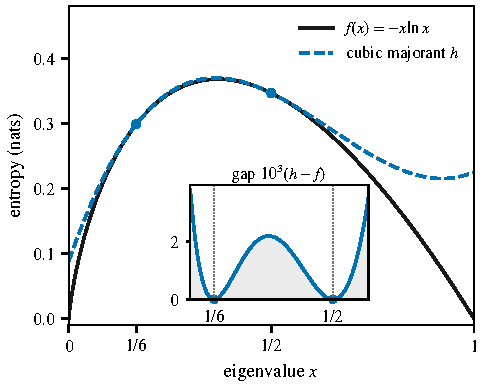
\includegraphics[width=0.5\linewidth]{fig_majorant}
\caption{The single-eigenvalue entropy contribution $f(x)=-x\ln x$ (in nats) and its cubic majorant $h$, tangent at the eigenvalues $1/6$ and $1/2$
of every cut of $M_4$. The inset magnifies the gap $h-f$ by $10^3$ on $[0.1,0.6]$: it is nonnegative, with double zeros at the nodes.
Summing $h$ over the cut spectra gives an affine upper bound on the entropy in terms of $P$ and $T$;
equality in this scalar bound requires every eigenvalue to be at a node.}
\label{fig:fqe-majorant}
\end{figure}

Return now to unit states. Each cut has four eigenvalues \(\lambda\) with \(\sum\lambda=1\),
\(\sum\lambda^2=\mathrm{tr}\rho_{1j}^2\), \(\sum\lambda^3=\mathrm{tr}\rho_{1j}^3\). Summing \(h\) over the 12
eigenvalues of the three cuts, \[
3\ln2\;E(\psi)=\sum_{j,\lambda}f(\lambda)=\kappa_0+bP+aT-\Delta_H,\qquad
\Delta_H=\sum_{j,\lambda}(h-f)(\lambda)\ge0,
\] with a constant \(\kappa_0\) independent of \(\psi\). At \(M_4\) every cut has spectrum
\((\tfrac12,\tfrac16,\tfrac16,\tfrac16)\), so \(\Delta_H=0\), \(P=1\), \(T=\tfrac5{12}\) and
\(E(M_4)=\tfrac12+\tfrac12\log_26=1+\tfrac12\log_23\). Subtracting, and using \(T=(17P-12-F)/12\)
(the definition of \(F\) at \(N=1\)), \[
\begin{aligned}
3\ln2\,\bigl(E(M_4)-E(\psi)\bigr)
&=-b(P-1)-a\bigl(T-\tfrac5{12}\bigr)+\Delta_H\\
&=\bigl(\tfrac{15}{2}-6\ln3\bigr)(P-1)
+\tfrac32(\ln3-1)F+\Delta_H.
\end{aligned}\tag{EG}\label{eq:fqe-entropy-gap}
\] Here \(-b-\tfrac{17}{12}a=\tfrac{15}2-6\ln3\) and \(a/12=\tfrac32(\ln3-1)\). All three terms
are nonnegative: \(\tfrac{15}2-6\ln3>0\) (since \(1<\ln3<5/4\)), \(P\ge1\)
(Lemma~\ref{lem:fqe-purity}), \(F\ge0\) (Theorem~\ref{thm:fqe-moment}), \(\Delta_H\ge0\). This
proves \(E(\psi)\le E(M_4)=1+\tfrac12\log_23\).

\paragraph{Why the bound is tight.} The entropy bound uses only the nonnegativity of $F$, rather than its stronger polarisation remainder. Its unit zeros are exactly the two
$M_4$ LU orbits and the three LU orbits of products of two Bell pairs, one for each pairing of the qubits
(Proposition~\ref{prop:fqe-moment-zeros} of Appendix~\ref{sec:fqe-sextic}). Only the two HS orbits saturate the entropy bound,
since products of two Bell pairs have $P=\tfrac32$. The cubic majorant touches the entropy function exactly at the eigenvalues of $M_4$, and
its coefficient signs make both moment slacks, $P-1$ and $F$, enter~\eqref{eq:fqe-entropy-gap} with nonnegative
weights. The same criterion yields the Tsallis bound for $0<q<2$ and the R\'enyi bound for $0<q<1$
(Proposition~\ref{prop:fqe-majorant}). At Tsallis order $q=2$ all critical states with $\tau=0$ tie.
Appendix~\ref{sec:fqe-correlation} gives a correlation-volume interpretation of the moment inequality. The sextic identity also
controls the spin flip: for unit states $F\ge\frac34W_1+\tau-\tau^{3/2}$ (Theorem~\ref{thm:fqe-general-envelope}), with equality on
product states and, for every $\tau\in[0,1]$, on a family of critical states. With the gap formula~\eqref{eq:fqe-entropy-gap}
this gives the Tsallis and von Neumann stability estimates in $W_1$ and $\tau$ of Appendix~\ref{sec:fqe-spectral-proofs}.

Being cubic in $|\psi\rangle\langle\psi|$, the sextic identity is a certificate at the three-copy level of the same
hierarchy, for the objective $F$ instead of a purity (Appendix~\ref{sec:fqe-seven}).

\subsection{Equality and one-cut rigidity}\label{sec:fqe-entropy_maximum-equality-and-one-cut-rigidity}

\begin{proposition}[one-cut rigidity]\label{prop:fqe-onecut} If $P=1$ and a $2|2$ cut has spectrum
$(1/2,1/6,1/6,1/6)$, then $\psi$ is LU-equivalent to $M_4$ or $\overline{M_4}$.

\end{proposition}

\begin{proof} Relabel the chosen cut as \(12|34\). Lemma~\ref{lem:fqe-purity} gives criticality and
\(\tau=0\). Write two-qubit states in the Bell basis with the phases of the magic basis,
\[
m_1=\tfrac1{\sqrt2}(|00\rangle+|11\rangle),\quad
m_2=\tfrac{i}{\sqrt2}(|01\rangle+|10\rangle),\quad
m_3=\tfrac1{\sqrt2}(|01\rangle-|10\rangle),\quad
m_4=\tfrac{i}{\sqrt2}(|00\rangle-|11\rangle),
\]
and a four-qubit state as \(\psi=\sum_{j,k}Z_{jk}\,m_j\otimes m_k\), with qubits \(1,2\) indexing the rows of \(Z\) and
qubits \(3,4\) the columns. In this basis single-qubit unitaries on each pair act, up to phase, as real four-dimensional rotations, so
local unitaries act by \(Z\mapsto O_1ZO_2^T\) with \(O_1,O_2\in SO(4)\). By the critical normal form
(Theorem~\ref{thm:fqe-critical-normal-form} of Appendix~\ref{sec:fqe-normal-form}), \(\psi\) is LU-equivalent to \(G(v)=\sum_kv_k\,m_k\otimes m_k\), that is
\(Z=\operatorname{diag}(v)\), with \(v\in\mathbb C^4\) a unit vector. The
cut spectrum and \(\tau\) are LU invariant (the latter by
\eqref{eq:fqe-spin-flip-normal-form}). On \(G(v)\) the spectrum of the cut \(12|34\) is
\(\{|v_k|^2\}\) (the \(m_k\) are orthonormal), and \(\tau=|\sum_kv_k^2|^2\) by
\eqref{eq:fqe-spin-flip-normal-form}.
Fix the large coordinate to \(1/\sqrt2\) by a common phase. Then \(\tau=0\) says that the other three
squares have modulus \(1/6\) and sum to \(-1/2\). Their sum has the largest possible modulus,
\(3(1/6)=1/2\), so equality in the triangle inequality forces all three squares to equal \(-1/6\). Thus, up to position of the large coordinate,
\[
 v=(\sqrt3,\pm i,\pm i,\pm i)/\sqrt6.
\]
The rotations \(Z\mapsto O_1ZO_2^T\) reduce these sign choices to two.
Applying the same determinant-one signed permutation on both sides of $G(v)$
moves the large entry to the first position without changing the other entries
except for their order. A diagonal rotation on one side can flip any pair of
small signs. Thus only their parity matters, giving the representatives
$(\sqrt3,i,i,i)/\sqrt6$ and $(\sqrt3,-i,-i,-i)/\sqrt6$.
Expanding the $m_k$ shows that
\[
 M_4=G\bigl((1,1,i\sqrt3,1)/\sqrt6\bigr).
\]
Multiplying by $-i$ and moving its third coordinate to the first gives the second representative.
Complex conjugation gives the first, since each $m_k\otimes m_k$ is a real vector, so $\overline{G(v)}=G(\bar v)$. Both representatives therefore belong to the stated pair
of LU orbits.
Relabelling preserves the pair of orbits, since it permutes the coefficient triple
\((1,\omega,\omega^2)\) up to common phase and conjugation.
\end{proof}

\emph{Proof of equality in Theorem~\ref{thm:fqe-entropy-max}.} Suppose $E(\psi)=E(M_4)$. The
positive coefficients in \eqref{eq:fqe-entropy-gap} force $P=1$ and $\Delta_H=0$.
The strict Hermite remainder above then forces every cut eigenvalue to be
$\tfrac16$ or $\tfrac12$. Four such eigenvalues with sum $1$ are
$(\tfrac12,\tfrac16,\tfrac16,\tfrac16)$, so Proposition~\ref{prop:fqe-onecut} applied to any one cut
shows that $\psi$ is LU-equivalent to $M_4$ or $\overline{M_4}$. This identifies the equality states without classifying all zeros
of $F$ or separately excluding Bell-pair products. Conversely, $M_4$ and its conjugate
have this spectrum on every cut and attain the bound. This proves Theorem~\ref{thm:fqe-entropy-max},
including equality.

\begin{remark}[a single orbit]\label{rem:fqe-single-orbit} The transposition of qubits $2$ and $3$
exchanges $|0011\rangle\leftrightarrow|0101\rangle$ and $|1100\rangle\leftrightarrow|1010\rangle$ and
fixes $|0110\rangle$ and $|1001\rangle$. It therefore sends the coefficient triple
$(1,\omega,\omega^2)$ of $M_4$ to $(\omega,1,\omega^2)=\omega\,(1,\omega^2,\omega)$, that is,
\[
M_4\longmapsto\omega\,\overline{M_4}.
\]
Since $E$ is invariant under qubit
permutations and $\omega$ is a global phase, the two local-unitary orbits of
Theorem~\ref{thm:fqe-entropy-max} are exchanged by a permutation of the qubits: the set of maximisers
is a single orbit under local unitaries together with qubit permutations. This is a special case of
the observation of Lyons, Arnold and Swogger~\cite{LAS}: even permutations of the qubits fix $M_4$ up to
phase, and odd ones map it to $\overline{M_4}$.
\end{remark}
